\section{Machine Learning}

\begin{definition}[\textit{Learning}]
    A computer program is said to learn from experience $E$ with respect to some class of tasks $T$ and performance measure $P$ if it improves with experience $E$. 
\end{definition}

Machine Learning derives knowledge from experience and induction.

In Machine Learning, we depend on computers to make informed decisions using new, unfamiliar data. 
Designing a comprehensive set of meaningful rules can prove to be exceedingly difficult. 
Machine Learning facilitates the automatic extraction of relevant insights from historical data and effectively applies them to new datasets.

The objective is to automate the programming process for computers, acknowledging the bottleneck presented by writing software.
Instead, our aim is to utilize the data itself to accomplish the required tasks.

\begin{figure}[H]
    \centering
    \begin{subfigure}{0.49\textwidth}
        \centering
        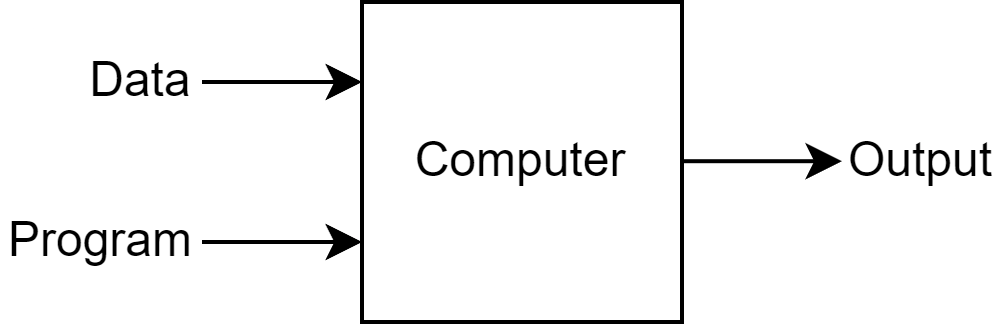
\includegraphics[width=0.9\linewidth]{images/program.png} 
        \caption{Programming}
    \end{subfigure}
    \begin{subfigure}{0.49\textwidth}
        \centering
        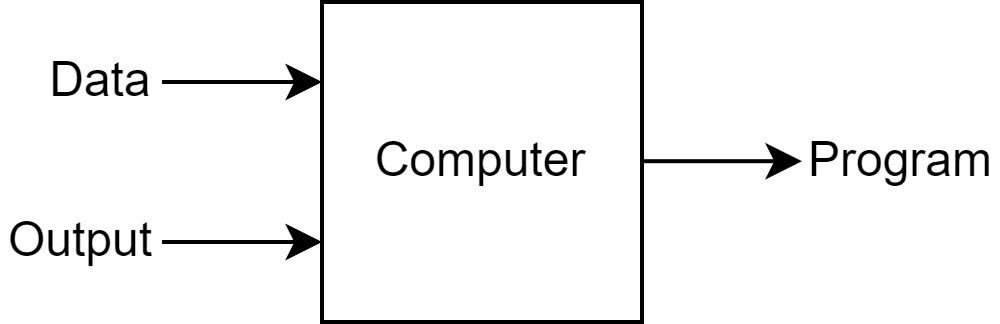
\includegraphics[width=0.9\linewidth]{images/learning.png}
        \caption{Machine Learning}
    \end{subfigure}
    \caption{Difference between programming and Machine Learning}
\end{figure}

Machine Learning paradigms can be categorized into three main types:
\begin{itemize}
    \item \textit{Supervised learning}: involves labeled data and direct feedback, aiming to predict outcomes or future events.
    \item \textit{Unsupervised learning}: operates without labeled data or feedback, focusing on discovering hidden structures within the data.
    \item \textit{Reinforcement learning}: centers around a decision-making process, incorporating a reward system to learn sequences of actions.
\end{itemize}